
% v2-acmsmall-sample.tex, dated March 6 2012
% This is a sample file for ACM small trim journals
%
% Compilation using 'acmsmall.cls' - version 1.3 (March 2012), Aptara Inc.
% (c) 2010 Association for Computing Machinery (ACM)
%
% Questions/Suggestions/Feedback should be addressed to => "acmtexsupport@aptaracorp.com".
% Users can also go through the FAQs available on the journal's submission webpage.
%
% Steps to compile: latex, bibtex, latex latex
%
% For tracking purposes => this is v1.3 - March 2012
\documentclass[prodmode,acmtecs]{acmsmall} % Aptara syntax
\usepackage[spanish,polish]{babel}
\usepackage[T1]{fontenc}
\usepackage{fancyvrb}
\usepackage{graphicx,hyperref}
\newcommand\cutout[1]{}


\usepackage[table]{xcolor}
\usepackage[utf8]{inputenc}
\usepackage[parfill]{parskip}
\usepackage{tabulary}
\PassOptionsToPackage{hyphens}{url}
\usepackage{hyperref}    
\usepackage[capitalize]{cleveref}


% Metadata Information
% !!! TODO: SET THESE VALUES !!!
\acmVolume{0}
\acmNumber{0}
\acmArticle{CFP}
\acmYear{0}
\acmMonth{0}

\newcounter{colstart}
\setcounter{page}{4}

\RecustomVerbatimCommand{\VerbatimInput}{VerbatimInput}%
{
%fontsize=\footnotesize,
fontfamily=\rmdefault
}


\newcommand{\UnderscoreCommands}{%\do\verbatiminput%
\do\citeNP \do\citeA \do\citeANP \do\citeN \do\shortcite%
\do\shortciteNP \do\shortciteA \do\shortciteANP \do\shortciteN%
\do\citeyear \do\citeyearNP%
}

\usepackage[strings]{underscore}



% Document starts
\begin{document}


\setcounter{colstart}{\thepage}

\acmArticle{CFP}
\title{{\huge\sc SIGLOG Monthly 263}

 July 2025}\author{ELLI ANASTASIADI\affil{Aalborg University, SE}\vspace*{-2.6cm}\begin{flushright}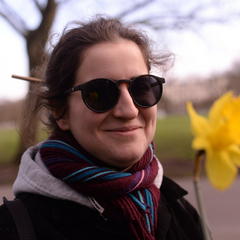
\includegraphics[width=30mm]{elli_anastasiadi.png}\end{flushright}}\begin{abstract}July 2025 edition of SIGLOG Monthly, featuring deadlines, calls and community announcements.
\end{abstract}


\maketitlee

\href{https://lics.siglog.org/newsletters/}{Past Issues}
 - 
\href{https://lics.siglog.org/newsletters/inst.html}{How to submit an announcement}
\section{Table of Contents}\begin{itemize}\item DEADLINES (\cref{deadlines}) 
 
\item CALLS 
 
\begin{itemize}\item SIR@IWCS2025 (CALL FOR PAPERS) (\cref{SIRIWCS2025})
\item PETER ACZEL MEMORIAL CONFERENCE \& BRITISH LOGIC COLLOQUIUM 2025 (CALL FOR PAPERS) (\cref{PETERACZELMEMORIALCONFERENCEBRITISHLOGICCOLLOQUIUM2025})
\item REACTS'25 (CALL FOR PAPERS) (\cref{REACTS25})
\item CPP 2026 (CALL FOR PAPERS) (\cref{CPP2026})
\item FoSSaCS 2026 (CALL FOR PAPERS) (\cref{FoSSaCS2026})
\item ICLP 2025 (CALL FOR PARTICIPATION) (\cref{ICLP2025})
\item WoLLIC 2025 (CALL FOR PARTICIPATION) (\cref{WoLLIC2025})
\item CONFEST 2025 (CALL FOR PARTICIPATION) (\cref{CONFEST2025})
\end{itemize} 
\item JOB ANNOUNCEMENTS 
 
\begin{itemize}\item Professor position (\cref{Professorposition})
\end{itemize} 
\end{itemize}\section{Deadlines}\label{deadlines}\rowcolors{1}{white}{gray!25}\begin{tabulary}{\linewidth}{LL}ICLP 2025:  & Jul 06, 2025 (Submission deadline) \\
SIR@IWCS2025:  & Jul 14, 2025 (Paper deadline) \\
CSL 2026:  & Jul 15, 2025 (Abstract), Jul 21, 2025 (Paper) \\
CONFEST 2025:  & Jul 26, 2025 (Early registration) \\
PETER ACZEL MEMORIAL CONFERENCE \& BRITISH LOGIC COLLOQUIUM 2025:  & Jul 31, 2025 (Abstracts deadline) \\
REACTS'25:  & Aug 13, 2025 (Abstract), Aug 20, 2025 (Paper) \\
CPP 2026:  & Sep 05, 2025 (Abstract Submission Deadline), Sep 12, 2025 (Paper Submission Deadline) \\
FoSSaCS 2026:  & Oct 16, 2025 (Submission deadline) \\
FM 2026:  & Nov 25, 2025 (Abstract Submission), Dec 02, 2025 (Full Paper Submission) \\
\end{tabulary}
\section{SIR@IWCS2025: First Workshop on Semantics for Interdisciplinary Research}\label{SIRIWCS2025}  Dusseldorf, Germany\\ 
  September 24 2025\\ 
  \href{https://team.inria.fr/semagramme/first-workshop-on-semantics-for-interdisciplinary-research/}{https://team.inria.fr/semagramme/first-workshop-on-semantics-for-interdisciplinary-research/}\\ 
  \href{https://openreview.net/group?id=inria.fr/INRIA/SC3A9magramme/2025/SIR01}{https://openreview.net/group?id=inria.fr/INRIA/SC3A9magramme/2025/SIR01}\\ 
CALL FOR PAPERS 

\begin{itemize}\item  In recent years, Natural Language Processing (NLP) has increasingly intersected with the humanities and social sciences, offering new methodologies for analyzing textual data, interpreting meaning, and modelling language-based phenomena. The potential for multi-disciplinary research using NLP methods is particularly great in computational semantics (CS), as its ability to process and represent meaning opens up innovative pathways for researchers in history, philosophy, literary studies, political science, etc.  This workshop aims to explore how semantic models and tools can be leveraged to tackle traditional and emerging questions in the Humanities in a broader sense (Social Sciences, Law, Economics, Management, Literature, Languages, Art, …). A major theme of  SIR is the role of semantics in NLP applied to the humanities (both statistical and symbolic approaches). 
 
\item  IMPORTANT DATES 
 
\rowcolors{1}{white}{gray!25}\begin{tabulary}{\linewidth}{LL}Paper deadline:  & July 14th (anywhere on earth) \\
Notification:  & August 25th (anywhere on earth) \\
Camera Ready:  & September 10th (anywhere on earth) \\
Workshop:  & September 24th (anywhere on earth) \\
\end{tabulary}
 
\item  Submission Information 
 
  Papers should describe original research and must not exceed 4 pages (with an extra page in the camera ready version for accepted papers). Papers should be submitted no later than 14 July 2025 (anywhere on earth). Accepted papers will be published in the conference proceedings in the ACL Anthology. For inclusion in the proceedings, at least one author must register to the conference and present the paper in person. Submissions should be fully anonymous to ensure double-blind reviewing. Submission via : \href{https://openreview.net/group?id=inria.fr/INRIA/SC3A9magramme/2025/SIR01}{https://openreview.net/group?id=inria.fr/INRIA/SC3A9magramme/2025/SIR01} . The workshop follow the IWCS 2025 template see the workshop web page. 
 
\item  ORGANISERS 
 
\begin{itemize}\item  Maxime Amblard, Université de Lorraine
\item  Ellen Breitholtz, Gothenburg University
\end{itemize} 
\item  CONTACT  
 
  maxime.amblard@univ-lorraine.fr and ellen.breitholtz@ling.gu.se 
 
\end{itemize}\section{PETER ACZEL MEMORIAL CONFERENCE \& BRITISH LOGIC COLLOQUIUM 2025 }\label{PETERACZELMEMORIALCONFERENCEBRITISHLOGICCOLLOQUIUM2025}  10-12 September 2025, Manchester, UK\\ 
  \href{https://sites.google.com/view/blc2025/home}{https://sites.google.com/view/blc2025/home}\\ 
CALL FOR PAPERS 

\begin{itemize}\item  The Peter Aczel Memorial Conference and the British Logic Colloquium 2025 meeting will be held at the University of Manchester (UK) on 10, 11, 12 September 2025.  
 
\item  Registration is open at: \href{https://estore.manchester.ac.uk/conferences-and-events/faculty-of-science-engineering/department-of-mathematics/departments-of-mathematics/british-logic-colloquium-2025-and-peter-aczel-memorial-conference}{https://estore.manchester.ac.uk/conferences-and-events/faculty-of-science-engineering/department-of-mathematics/departments-of-mathematics/british-logic-colloquium-2025-and-peter-aczel-memorial-conference} 
 
\item  The programme committee invites abstracts for Contributed Talks. Students and early-career researchers are especially encouraged to present their work.  
 
\item  IMPORTANT DATES 
 
Abstracts deadline: Jul 31, 2025 
 
\item  Invited speakers for the Peter Aczel memorial conference (10 September): 
 
\begin{itemize}\item  Steve Awodey (Carnegie Mellon University),
\item  Jouko Vaananen (University of Helsinki),
\item  Rosalie Iemhoff (Utrecht University),
\item  Andrew Swan (University of Ljubljana),
\end{itemize} 
\item  Invited speakers for the BLC meeting (11-12 September) are: 
 
\begin{itemize}\item  Mirna Dzamonja (Paris),
\item  Fairouz Kamareddine (Heriot-Watt),
\item  Fraser MacBride (Manchester),
\item  Paul-André Melliès (Paris),
\item  Paula Quinon (Lund/Warsaw),
\item  Katrin Tent (Münster),
\item  Frank Wolter (Liverpool)
\end{itemize} 
\item  Additional information is available from: \href{https://sites.google.com/view/blc2025/home}{https://sites.google.com/view/blc2025/home} 
 
\end{itemize}\section{REACTS'25: International Workshop on Reconfigurable Transition Systems: Semantics, Logics and Applications}\label{REACTS25}  \href{https://reacts-workshop.github.io/2025/}{https://reacts-workshop.github.io/2025/}\\ 
  Tuesday, 10-11 November 2025\\ 
  Toledo, Spain\\ 
  Satellite event of SEFM 2025 (\href{https://sefm-conference.github.io/sefm2025}{https://sefm-conference.github.io/sefm2025})\\ 
CALL FOR PAPERS 

\begin{itemize}\item  OVERVIEW 
 
  Reconfigurable Transition Systems (RTS) are dynamic relational structures (graphs) that evolve along its execution, in the sense that their accessibility relation, their set of nodes or their labelling change when their edges are crossed. These structures have proven to be suitable to compactly represent complex reactive and reconfigurable behaviours. Namely, the ability of reacting or readapting under the influence of certain events is a very distinctive feature of many diverse situations and objects. An autonomous vehicle that changes its route due to a new strike occurring, the behaviour of a software component after a memory disposal, or a DNA mutation as the result of a viral infection, are different examples that witness the importance of modelling about changes in a determined situation. Practical user cases have aroused the interest of the logic community in the study of variants of RTS, by developing formal methods to properly reason about such situations. 
 
  This workshop aims to bring together the whole community of researchers working on different ways to model reconfigurable and reactive systems from a formal perspective. This includes theoretical approaches (like hybrid logics, reactive frames, model-update logics, and topological and algebraic semantics), or formalisms designed for specific purposes (like separation logic in software verification, dynamic epistemic logic in AI planning, and others). Also, our goal is to devise novel approaches and potential applications, and share a common perspective on the discipline. 
 
\item  SUBMISSION GUIDELINES 
 
  Authors are invited to submit, via CMT, research contributions or experience reports (\href{https://cmt3.research.microsoft.com/reacts2025}{https://cmt3.research.microsoft.com/reacts2025}). All papers should be written in English and prepared using the specific LNCS templates available at \href{http://www.springer.de/comp/lncs/authors.html}{http://www.springer.de/comp/lncs/authors.html}. There are two categories of submissions: 
 
\begin{itemize}\item  FULL PAPERS up to 12 pages (excluding references) – to present original research and the analysis, interpretation and validation of the research findings.
\item  SHORT PRESENTATIONS up to 4 pages (excluding references) – to present work in progress and preliminary results.
\end{itemize} 
  Both kinds of submissions allow system descriptions,  to present a new tool, a new tool component or novel extensions to an existing tool aiming at supporting open community approaches, or the use/customisation of an existing tool in the context of RTS. Accepted full papers will be included in the workshop programme and will appear in the workshop LNCS proceedings. Accepted short presentations will be included in the pre-proceeding (available online before the Workshop) but not published in the LNCS proceedings. 
 
\item  PROGRAM CO-CHAIRS 
 
\begin{itemize}\item  José Proença, University of Porto (Portugal)
\item  Umberto Rivieccio, Universidad Nacional de Educación a Distancia (Spain)
\end{itemize} 
\item  PUBLICATION 
 
  Accepted full papers will be published by Springer in a volume of Lecture Notes in Computer Science (\href{http://www.springer.com/lncs}{http://www.springer.com/lncs}), which will collect contributions to some workshops co-located with SEFM 2025. Condition for inclusion in proceedings is that at least one of the co-authors has presented the paper at the Workshop. Similarly to the last edition of ReacTS, we plan to invite authors of selected contributions to submit extended versions to a special issue, e.g. to the Journal of Applied Logics. 
 
\item  IMPORTANT DATES 
 
\rowcolors{1}{white}{gray!25}\begin{tabulary}{\linewidth}{LL}Abstract submission:  & Aug 13, 2025 \\
Paper submission:  & Aug 20, 2025 \\
Author notification:  & Sep 22, 2025 \\
Workshop:  & Nov 10-11, 2025 \\
\end{tabulary}
 
\item  CONTACT 
 
  If you have any problems or questions, please contact us via e-mail at: jose.proenca@fc.up.pt / umberto@fsof.uned.es 
 
\end{itemize}\section{CPP 2026: Certified Programs and Proofs}\label{CPP2026}  \href{https://popl26.sigplan.org/home/CPP-2026}{https://popl26.sigplan.org/home/CPP-2026}\\ 
  Rennes, France\\ 
  12-13 January 2025\\ 
CALL FOR PAPERS 

\begin{itemize}\item  Certified Programs and Proofs (CPP) is an international conference on practical and theoretical topics in all areas that consider formal verification and certification as an essential paradigm for their work. CPP spans areas of computer science, mathematics, logic, and education. CPP 2026 (\href{https://popl26.sigplan.org/home/CPP-2026}{https://popl26.sigplan.org/home/CPP-2026}) will be held on 12-13 January 2025 and will be co-located with POPL 2026 in Rennes, France. CPP 2026 is sponsored by ACM SIGPLAN, in cooperation with ACM SIGLOG. CPP 2026 will welcome contributions from all members of the community. The CPP 2026 organizers will strive to enable both in-person and remote participation, in cooperation with the POPL 2026 organizers. 
 
\item  IMPORTANT DATES 
 
\rowcolors{1}{white}{gray!25}\begin{tabulary}{\linewidth}{LL}Abstract Submission Deadline:  & Sep 05, 2025 \\
Paper Submission Deadline:  & Sep 12, 2025 \\
Notification (tentative):  & Nov 13, 2025 \\
Camera Ready Deadline (tentative):  & Dec 01, 2025 \\
Conference:  & Jan 12-13, 2026 \\
\end{tabulary}
 
  Deadlines expire at the end of the day, anywhere on earth. Abstract and submission deadlines are strict and there will be no extensions. 
 
\item  DISTINGUISHED PAPER AWARDS 
 
  Around 10% of the accepted papers at CPP 2026 will be designated as Distinguished Papers. This award highlights papers that the CPP program committee thinks should be read by a broad audience due to their relevance, originality, significance and clarity. 
 
\item  For a complete list of topics of interest, and detailed submission instructions, please visit the conference website.  
 
\item  ORGANIZERS 
 
\begin{itemize}\item  Kathrin Stark, Heriot-Watt University (conference co-chair)
\item  Yannick Zakowski, ENS Lyon (conference co-chair)
\item  Nikhil Swamy, Microsoft Research (PC co-chair)
\item  Nicolas Tabareau, Inria (PC co-chair)
\end{itemize} 
  For any questions please contact the two PC chairs: 
 
\begin{itemize}\item  Nikhil Swamy nswamy@microsoft.com
\item  Nicolas Tabareau nicolas.tabareau@inria.fr
\end{itemize} 
\end{itemize}\section{FoSSaCS 2026: 29TH INTERNATIONAL CONFERENCE ON FOUNDATIONS OF SOFTWARE SCIENCE AND COMPUTATION STRUCTURES (FoSSaCS 2026)}\label{FoSSaCS2026}  Part of the International Joint Conferences On Theory and Practice of  Software (ETAPS 2026)\\ 
  \href{https://etaps.org/2026/conferences/fossacs/}{https://etaps.org/2026/conferences/fossacs/}\\ 
  April 11-16, 2026\\ 
  Turin, Italy\\ 
CALL FOR PAPERS 

\begin{itemize}\item  GENERAL 
 
  FoSSaCS seeks original papers on foundational research with a clear significance for software science. The conference invites submissions on theories and methods to support the analysis, integration, synthesis, transformation, and verification of programs and software systems. 
 
\item  PROCEEDINGS 
 
  The FoSSaCS 2026 proceedings will be published in Springer LNCS as gold open access. 
 
\item  SUBMISSIONS 
 
  FoSSaCS solicits just a single paper category: research papers. The page limit is 18 pp excluding references, respecting Springer’s LNCS format at the submission time. Additional material (no page limit) can be placed in a clearly marked appendix, at the end of the paper.  The papers can be submitted at \href{https://easychair.org/conferences/?conf=fossacs2026}{https://easychair.org/conferences/?conf=fossacs2026} . FoSSaCS 2026 will adopt a double-blind reviewing process, in line with the other ETAPS conferences. PC members will be allowed to submit up to one paper. These submissions will be held to a higher standard - for example, PC submissions will not be part of the final vote. 
 
\item  ARTIFACT EVALUATION 
 
  FoSSaCS 2026 will have a post-paper-acceptance voluntary artifact evaluation. Authors will be encouraged to submit artifacts for evaluation after paper notification. The outcome will not alter the paper’s acceptance decision. Guillermo Alberto Perez (University of Antwerp) will act as the FoSSaCS artifact  evaluation chair. Detailed information will shortly appear at \href{https://etaps.org/2026/conferences/ae-esop-fase-fossacs}{https://etaps.org/2026/conferences/ae-esop-fase-fossacs} 
 
\item  IMPORTANT DATES 
 
\rowcolors{1}{white}{gray!25}\begin{tabulary}{\linewidth}{LL}Submission deadline:  & Oct 16, 2025 \\
Rebuttal:  & Dec 08, 2025 \\
Paper notification:  & Dec 22, 2025 \\
Voluntary artifact submission deadline:  & Jan 08, 2026 \\
Paper final version:  & Jan 22, 2026 \\
Artifact notification:  & Feb 12, 2026 \\
Main Conference:  & Apr 13–16, 2026 \\
\end{tabulary}
 
\item  PC CHAIRS 
 
\begin{itemize}\item  Nathalie Bertrand (Inria Rennes, France)
\item  Stefan Milius (Friedrich-Alexander Universität Erlangen-Nürnberg, Germany)
\end{itemize} 
\end{itemize}\section{ICLP 2025: 41st International Conference on Logic Programming }\label{ICLP2025}  University of Calabria, Rende, Italy\\ 
  September 12-19, 2025\\ 
CALL FOR PARTICIPATION 

\begin{itemize}\item  We are pleased to announce the availability of student grants to support participation in ICLP 2025, generously provided by the Artificial Intelligence Journal (AIJ), the Italian Association for Artificial Intelligence (AIxIA), and the Gruppo Ricercatori e Utenti Logic Programming (GULP). We encourage all eligible students to apply! 
 
\item  IMPORTANT DATES 
 
\rowcolors{1}{white}{gray!25}\begin{tabulary}{\linewidth}{LL}Submission deadline:  & Jul 06, 2025 \\
Notification of acceptance:  & Jul 13, 2025 \\
\end{tabulary}
 
\item  Who can apply? 
 
  Grants are available to Master’s and PhD students and are conditional upon: 
 
\begin{itemize}\item  A certificate of student status
\item  A statement confirming the lack of sufficient funds to attend ICLP 2025
\end{itemize} 
\item  What is covered? 
 
  The grants will partially cover registration fees and/or shared accommodation in university residences or nearby lodging facilities. The applicant can indicate the type of support he needs. AIJ offers multiple grants, which will be provided as direct discounts on conference services. AixIA offers two grants, up to 400 EUR each, which will be provided via reimbursement handled by the association after the conference.  GULP offers two grants, up to 260 EUR each, which will be provided via reimbursement handled by the association after the conference. For US-based students, an NSF-sponsored grant may become available later. Applicants should indicate their preference for a specific grant type in the application form. 
 
\item  Evaluation Criteria 
 
  Applications will be evaluated based on: 
 
\begin{itemize}\item  Whether the student is an author of a paper accepted at any ICLP-related event
\item  The submission timestamp
\item  Whether the applicant is a member of AIxIA or GULP Associations
\item  The personal preference for a specific grant
\end{itemize} 
  Under no circumstances can a grant be awarded to an applicant who is not enrolled in a recognized study program (Master’s level – ISCED Level 7 or PhD level – ISCED Level 8 or equivalent), or who is unable to provide valid proof of student status. The committee will maximise student participation given the available funds. If the NSF-sponsored grant becomes available, it will be allocated to eligible students based in the United States. 
 
  To apply, please complete the application form by July 6th by filling in the following form: \href{https://forms.gle/8w39MENkZ9nYbjo38}{https://forms.gle/8w39MENkZ9nYbjo38} 
 
\end{itemize}\section{WoLLIC 2025: 31st Workshop on Logic, Language, Information and Computation}\label{WoLLIC2025}  14-17 July 2025\\ 
  Porto, Portugal\\ 
  \href{https://wollic2025.github.io/}{https://wollic2025.github.io/}\\ 
CALL FOR PARTICIPATION 

\begin{itemize}\item  REGISTRATION 
 
  Registration is open in: \href{https://forms.gle/GKzvG4vTCEcxhgpS6}{https://forms.gle/GKzvG4vTCEcxhgpS6} 
 
\begin{itemize}\item  Late registration:
\item Regular: 360 euros
\item Student: 310 euros
\end{itemize} 
\item  INVITED SPEAKERS 
 
\begin{itemize}\item  Tobias Kappé (Leiden University): On propositional program equivalence.
\item  Daniela Petrişan (IRIF, Université de Paris): Functorial Mealy machines.
\end{itemize} 
\item  ACCEPTED PAPERS 
 
  The list of accepted papers can be found at \href{https://wollic2025.github.io/accepted/}{https://wollic2025.github.io/accepted/} 
 
\item  WoLLIC is an annual international forum on interdisciplinary research involving formal logic, computing and programming theory, and natural language and reasoning. Each meeting includes invited talks and tutorials as well as contributed papers. The thirty-first WoLLIC will be held at the University of Porto, Portugal, 14-17 July 2025. WoLLIC is a series of workshops which started in 1994 with the aim of fostering interdisciplinary research in pure and applied logic. The idea is to have a forum which is large enough in the number of possible interactions between logic and the sciences related to information and computation, and yet is small enough to allow for concrete and useful interaction among participants. 
 
\item  SCIENTIFIC SPONSORSHIP 
 
\begin{itemize}\item  Interest Group in Pure and Applied Logics (IGPL)
\item  The Association for Logic, Language and Information (FoLLI)
\item  Association for Symbolic Logic (ASL)
\item  European Association for Theoretical Computer Science (EATCS)
\item  European Association for Computer Science Logic (EACSL)
\item  Sociedade Brasileira de Lógica (SBL)
\item  Sociedade Portuguesa de Lógica (SPL)
\end{itemize} 
\end{itemize}\section{CONFEST 2025: CONCUR, FMICS, QEST\_FORMATS}\label{CONFEST2025}  \href{https://conferences.au.dk/confest2025}{https://conferences.au.dk/confest2025}\\ 
  CONCUR, FMICS, QEST+FORMATS, and six co-located workshops\\ 
  August 25-30, 2025\\ 
  Aarhus, Denmark\\ 
CALL FOR PARTICIPATION 

\begin{itemize}\item  OVERVIEW 
 
\begin{itemize}\item  8 invited talks
\item  75 conference paper presentations
\item  6 co-located workshops
\end{itemize} 
  The early registration deadline is July 26, 2025. 
 
  We are excited to invite you to register for CONFEST 2025, which will host three major international conferences: 
 
\begin{itemize}\item  CONCUR 2025: 36th International Conference on Concurrency Theory
\item  FMICS 2025: 30th International Conference on Formal Methods for Industrial Critical Systems
\item  QEST+FORMATS 2025: Joint International Conference on Quantitative Evaluation of Systems and Formal Modeling and Analysis of Timed Systems
\end{itemize} 
  These events will take place in Aarhus, Denmark, from August 25 to August 30, offering a fantastic opportunity to follow the latest advancements, and network with researchers and practitioners in these fields. For more information about the conferences and the venue, please visit: \href{https://conferences.au.dk/confest2025}{https://conferences.au.dk/confest2025} 
 
\item  Registration 
 
  The Early Registration deadline is  
 
Early registration: Jul 26, 2025 
 
  via: \href{https://conferences.au.dk/confest2025/registration}{https://conferences.au.dk/confest2025/registration} 
 
  Some hotel booking codes are available here: \href{https://conferences.au.dk/confest2025/hotel-accommodations}{https://conferences.au.dk/confest2025/hotel-accommodations} . Other accommodation options are available here: \href{https://www.visitaarhus.com/aarhus/where-sleep/hotels}{https://www.visitaarhus.com/aarhus/where-sleep/hotels} 
 
\item  Invited Speakers 
 
\begin{itemize}\item  Alessandro Abate, U of Oxford, UK. Title: Neural synthesis for verification and control of stochastic systems - certificates and abstractions
\item  Christel Baier, TU Dresden, Germany. Title: Linear Temporal Logic with Standpoint Modalities
\item  Lu Feng, University of Virginia, USA. Title: Runtime Safety for Learning-Enabled Cyber-Physical Systems: From Predictive Monitoring to Adaptive Shielding
\item  Arnd Hartmanns, U of Twente, NL. Title: Sound and Modest Approaches to Quantitative Model Checking from Sea to Space
\item  Chris Heunen, U of Edinburgh, UK. Title: Towards categorical quantum concurrency theory
\item  Christoph Matheja, U of Oldenburg, Germany and DTU Denmark. Title: Automating Proof Rules for Probabilistic Programs
\item  Ina Schieferdecker, Independent Researcher, Germany. Title: Empowering Testing with AI - Navigating the growing field of research on AI for software testing
\item  Jiri Srba, Aalborg University, Denmark. Title: On-the-Fly Verification: Advancements in Dependency Graphs
\end{itemize} 
\item  Workshops 
 
\begin{itemize}\item  BMQL 2025 - 1st IW on Behavioural Metrics and Quantitative Logics
\item  Express/SOS 2025 - combined IW on Expressiveness in Concurrency and Structural Operational Semantics
\item  FMQC 2025 - IW on Formal Methods in Quantum Computing
\item  PFQA 2025 - Colloquium on Principles of Formal Quantitative Analysis
\item  Radical 2025 -  4th IW on Recent Advances in Concurrency and Logic
\item  SynCoP 2025 - 10th IW on Synthesis of Complex Parameters
\end{itemize} 
  We hope to meet you in Aarhus this summer! 
 
\end{itemize}\section{Professor position: Roskilde University, Denmark}\label{Professorposition}JOB ANNOUNCEMENT 

\begin{itemize}\item  Roskilde University, Denmark, invites applications for a Professor of Computer Science or Associate Professor on the promotion programme of Computer Science. 
 
\item  We are seeking applicants with a background in Computer Science and a strong research profile in Data Science, preferably within the domain of Machine Learning. We are particularly interested in applicants with research in one or more of the following subject areas: (1) explainable AI, (2) the combination machine learning and symbolic reasoning, (3) language models or Natural Language Processing, and (4) cybersecurity. 
 
\item  Application deadline: September 7th, 2025. 
 
\item  For more information, see: \href{https://candidate.hr-manager.net/ApplicationInit.aspx?cid=1310\&ProjectId=147722}{https://candidate.hr-manager.net/ApplicationInit.aspx?cid=1310\&ProjectId=147722} 
 
\end{itemize}


\bigskip Links: \href{http://siglog.org/}{SIGLOG website}, \href{https://lics.siglog.org}{LICS website}, \href{https://lics.siglog.org/newsletters/}{SIGLOG Monthly}\end{document}